\begin{enumerate}[a.]
    \item ($\implies$) Assume that $D$ is not strongly connected. Then there exists $u, v \in V(D)$ such that there is no $u-v$ path in $D$. Then $d(u, v) = \infty = \max\{d(u, v) : v \in V(D)\}$. So $D$ has infinite-eccentricity. \\
    ($\impliedby$) Assume that $D$ is strongly connected. Let $u \in V(D)$ then for every $v \in V(D)$ there exists a $u-v$ path since $D$ is strongly connected and $d(u, v)$ is finite (the length of the minimum $u-v$ path and we know there's at least one). $\implies$ every vertex has finite eccentricity. 
    \item 
        \begin{enumerate}[(i)]
            \begin{figure}[H]
            \centering
            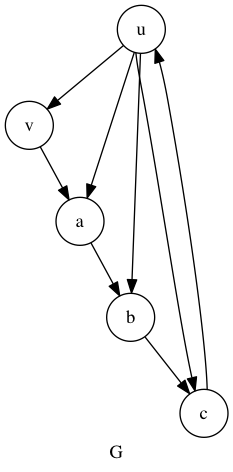
\includegraphics[scale=0.5]{218.png}
            \end{figure}
            \item From the figure above we can see that  $$e^+(u) = \max \{d(u, x) : x \in V(G)\} = 1$$ and $$e^+(v) = \max \{d(v, x) : x \in V(G)\} = 3$$ 
                So $|e^+(u) - e^+(v)| = 2 > 1$. 
                Disproving the question.
            \item Relabeling the figure above by swapping $u$ and $v$ then 
             $$e^+(v) = \max \{d(v, x) : x \in V(G)\} = 1$$ and $$e^+(u) = \max \{d(u, x) : x \in V(G)\} = 3$$ 
                So $|e^+(u) - e^+(v)| = |1 - 3| = |-2| = 2 > 1$
        \end{enumerate}
\end{enumerate}
